% !TEX encoding = UTF-8 Unicode
\documentclass[a4paper, 9pt, DIV=20]{scrartcl}
\usepackage[utf8]{inputenc}

\usepackage[swissgerman]{babel}
\usepackage{amsmath}
\usepackage{amsfonts}
\usepackage{amssymb}
\usepackage{mathtools}
\usepackage{pdfpages}
\usepackage{graphicx}
\usepackage{hyperref}

\usepackage{fancyhdr}

\usepackage{enumitem}

\title{Datenstrukturen und Algorithmen -- Zusammenfassung}
\author{David Bimmler}

\DeclareMathOperator{\clos}{clos}
\DeclareMathOperator{\Int}{int}
\DeclareMathOperator{\arcsinh}{arcsinh}
\DeclareMathOperator{\arccosh}{arccosh}
\DeclareMathOperator{\arctanh}{arctanh}
\DeclareMathOperator{\grad}{grad}
\DeclareMathOperator{\rot}{rot}
\DeclareMathOperator{\Div}{div}
\DeclarePairedDelimiter{\floor}{\lfloor}{\rfloor}
\DeclarePairedDelimiter{\ceil}{\lceil}{\rceil}

\newcommand{\N}{\mathbb{N}}
\newcommand{\R}{\mathbb{R}}
\newcommand{\C}{\mathbb{C}}
\newcommand{\Oh}{\mathcal{O}}
\newcommand{\Th}{\Theta}
\newcommand{\defeq}{\vcentcolon=}
\newcommand{\eqdef}{=\vcentcolon}

\begin{document}
\pagestyle{fancy}
\fancyhf{}
\fancyhead[L]{Zusammenfassung Datenstrukturen und Algorithmen}
\fancyhead[R]{David Bimmler, B.\ Sc.\ ETH Informatik, Legi-Nr.: 13-926-696 -- S. \thepage}

\begin{twocolumn}
\tableofcontents
\end{twocolumn}

\clearpage


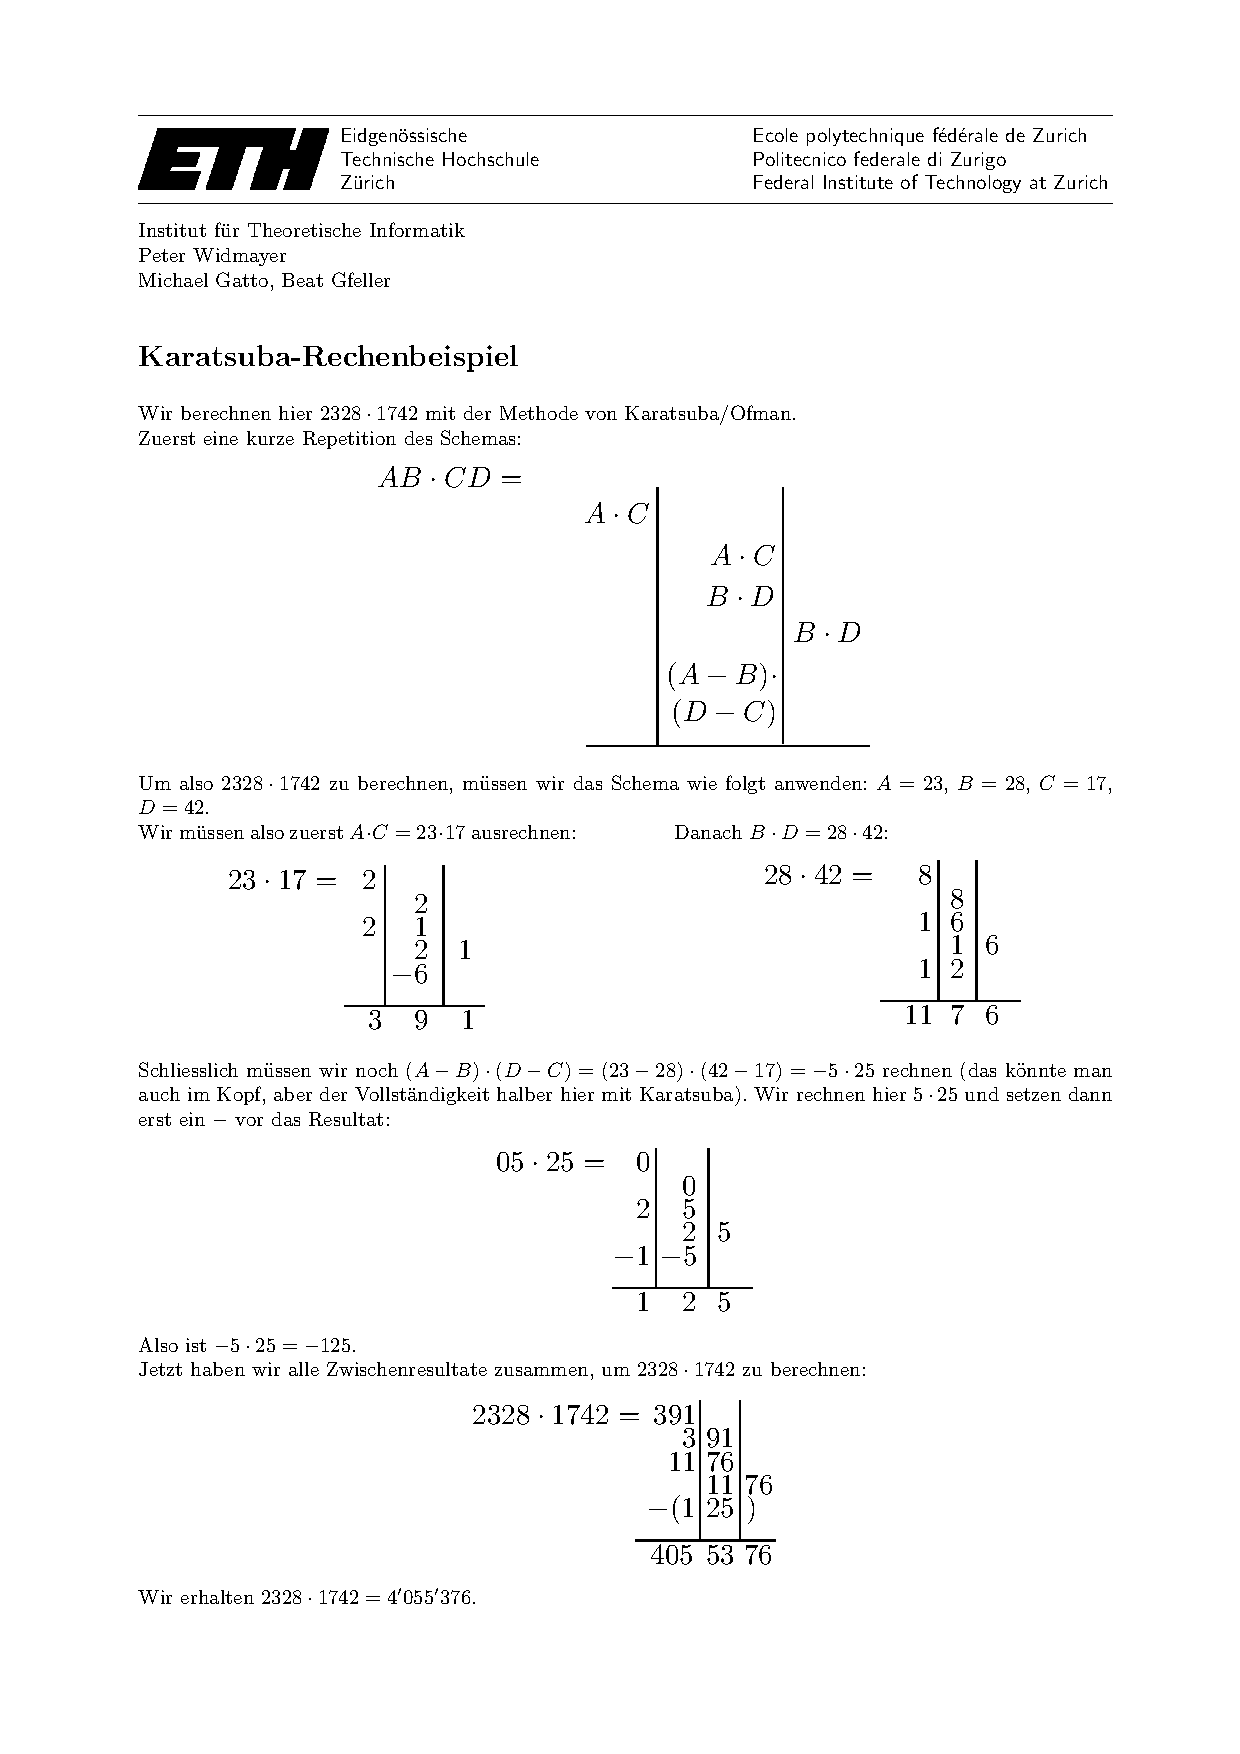
\includepdf[pages={-}]{Karatsuba.pdf}

\section{Algorithmen}

\subsection{$\Oh$-Notation}
Hier immer $f:\N\to\R^{+}$!
\begin{description}
\item[Obere Schranke] $ \mathcal O(g) \defeq \{f\,|\,\exists c\in\R^{+}, n_{0} \in\N\;\forall n \geq n_{0}:f(n) \leq cg(n)\} $
\item[Untere Schranke] $ \Omega(g) \defeq \{f\,|\,\exists c\in\R^{+}, n_{0} \in \N\;\forall n \geq n_{0}:f(n) \geq cg(n)\} $
\item[Asymptotisch gleich] $ \Theta(g) \defeq \{f\,|\,\exists c\in\R^{+}, n_{0} \in \N\;\forall n \geq n_{0}:  c^{-1}g(n) \leq f(n) \leq cg(n)\} $
\end{description}
\paragraph{Wachstumsordnung}
\[ 1 << \log\log n << \frac{\log n}{\log\log n} << \log n << \log^{2} n << \sqrt{n}\]
\[ n << n \log n << n^{1+\varepsilon} << n^{2} << n^{3} << c^{n} << n! << n^{n}\]

\subsection{Amortisierte Analyse}
Die tatsächlichen Kosten der $i$-ten Operation heissen $t_{i}$. Die Potentialfunktion $\Phi_{i}$ beschreibt das Potential nach der $i$-ten Operation. Demnach sind die amortisierten Kosten der $i$-ten Operation definiert als $a_{i}=t_{i}+\Phi_{i}-\Phi_{i-1}$. Damit folgt für $m$ Operationen: \[ \sum_{i=1}^{m}{a_{i}} = \sum_{i=1}^{m}{(t_{i}+\Phi_{i}-\Phi_{i-1})} = \Bigg( \sum_{i=1}^{m}{t_{i}}\Bigg) + \Phi_{m} - \Phi_{0}\]
Und dann \[ \sum_{i=1}^{m}{t_{i}} = \sum_{i=1}^{m}{a_{i}} - \Phi_{m} + \Phi_{0} \]
Wenn es also gelingt, die amortisierten Kosten und den Term $\Phi_{0} - \Phi_{m}$ abzuschätzen, hat man auch eine Abschätzung für die tatsächlichen Kosten. Wenn man dann noch $\Phi_{0} \leq \Phi_{m}$ hat, sind die amortisierten Kosten eine obere Schranke für die tatsächlichen Kosten.

\subsection{Dynamische Programmierung}
\begin{enumerate}
\item \emph{Definition der DP-Tabelle:} Welche Dimension hat die Tabelle? Was ist die Bedeutung jedes Eintrags?
\item \emph{Berechnung eines Eintrags:} Wie berechnet sich ein Eintrag aus den Werten von anderen Einträgen? Welche Einträge hängen nicht von anderen Einträgen ab?
\item \emph{Berechnungsreihenfolge:} In welcher Reihenfolge kann man die Einträge berechnen, so dass die jeweils benötigten anderen Einträge bereits vorher berechnet wurden?
\item \emph{Auslesen der Lösung:} Wie lässt sich die Lösung am Ende aus der Tabelle auslesen?
\end{enumerate}

\subsection{Sortieren}
\paragraph{Selectionsort} funktioniert via Auswählen der Position des minimalen Schlüssels $j_{1}$ und nachfolgigem Vertauschen von $a[1]$ mit $a[j_{1}]$. Dann wird $j_{2}$ bestimmt, und $a[j_{2}]$ mit $a[2]$ vertauscht, etc. Kann stabil implementiert werden. In-place.\\
$\Th(n^{2})$ Vergleiche, $\Th(n)$ Vertauschungen.

\paragraph{Insertionsort} Die zu sortierenden Elemente werden nacheinander betrachtet und in die jeweils bereits sortierte, anfangs leere Teilfolge an der richtigen Stelle eingefügt. Wenn also $a[1]$ bis $a[i-1]$ schon sortiert sind, wird $a[i]$ nach links verschoben, bis es am richtigen Platz ist. Stabil. In-place.\\
$\Oh(n^{2})$ Vergleiche und Vertauschungen

\paragraph{Shellsort} Wie Insertionsort, aber versucht das die Verschiebungsschritte zu vergrössern, indem eine Folge abnehmender Inkremente (z.B. $5,3,1$) verwendet wird. Eine Teilfolge kann dann $5$-sortiert sein. Nicht stabil. In-place. Bounds sind abhän-gig von der Inkrementenfolge.

\paragraph{Bubblesort} Verwendet als Bewegung \emph{nur} das Vertauschen benachbarter Datensätze. Läuft durch, und nimmt immer das grössere Element von zwei benachbarten mit. Stabil. In-place. \\
$\Oh(n^{2})$ Vertauschungen und Vergleiche.

\paragraph{Quicksort} Sortieren durch rekursives Teilen. Ein Pivotelement $k$ wird gewählt, mithilfe dessen die Elemente in zwei Teile geteilt werden. Die Elemente werden so um $k$ angeordnet (durch Vertauschen), dass das Problem jetzt nur noch aus dem Sortieren der zwei Teilfolgen besteht. Nicht stabil. In-place (abgesehen vom Rekursionsstack). $\Oh(n\log{n})$ Zeit.

\paragraph{Heapsort} Heap herstellen. Das kleinste (erste) Element ist das nächste in der Ordnung. Entferne es, und stelle die Heapbedingung für die restlichen Schlüssel wieder her. Nicht stabil. In-place. \\
$\Th(n\log{n})$ Zeit.

\paragraph{Mergesort} Die Gesamtfolge wird in zwei Teilfolgen geteilt, die rekursiv mit Mergesort sortiert werden. Danach werden die beiden Teilfolgen wieder zu einer Folge verschmolzen, indem man zwei Zeiger auf die ersten Elemente setzt, das kleinere der beiden nimmt und den Zeiger vorrückt. Natürlicher Mergesort versucht, schon existierende \hyperref[bitonische_laufe]{bitonische Läufe} auszunutzen. Stabil. Nicht in-place. \\
$\Th(n\log{n})$ Zeit.

\subsubsection{Radixsorts}
Radixsorts nutzen Eigenschaften neben Vergleichbarkeit der Schlüssel aus. Schlüssel sind Wörter über einem aus $m$ Elementen bestehenden Alphabet, also bei z.B. $m=10$ Dezimalzahlen, $m=2$ Binärzahlen.

\paragraph{Radix-exchange-sort} startet beim MSB, teilt die Folge in zwei und ruft sich rekursiv auf den beiden Teilfolgen auf. Dort wird dann aufgrund des nächsten Bits geteilt, etc. Geteilt wird wie bei Quicksort, zwei Zeiger laufen über die Schlüssel und vertauschen wenn nötig. Stabil. In-place. \\
$\Oh(n * b)$. Gut, wenn Anzahl Bits $b = \log{n}$. Nicht gut bei wenigen, langen Schlüsseln.

\paragraph{Bucketsort} Verteilungsphase: Schlüssel werden basierend auf der least-significant Ziffer auf Buckets verteilt (also $14, 24, 64, 44$ in einen Bucket). Sammelphase: Die Schlüssel werden eingesammelt, nach Bucket sortiert, innerhalb der Buckets das ``unterste'' zuerst. Es folgt eine Verteilphase basierend auf der nächsten Ziffer, und ebenso eine Sammelphase. Während der zweiten Verteilphase bleibt die Ordnung der ersten erhalten, die kleinsten least-significant Ziffern sind ``unten''. Stabil. Nicht in-place. \\
$\Oh(n+k)$ Laufzeit, mit $k$ Anzahl Buckets. Mit $k$ konstant $\Oh(n)$.

\subsection{Suchen}
\paragraph{Median der Mediane} ist ein Vorgehen, mit dem ein günstiges Pivot-Element gefunden werden kann. Man teilt die $N$ Elemente in $\floor{\frac{N}{5}}$ Gruppen auf, sortiert in diesen Gruppen in konstanter Zeit und wendet dieses Verfahren rekursiv auf die Mediane der 5er Gruppen an. Man erhält den Median der Mediane, welcher man als Pivot verwenden kann.

\paragraph{Auswahl} Mit dem Median der Mediane als gutes Pivot-Element kann das $i$-te Element einer Folge in $\Oh(n)$ gefunden werden.

\paragraph{Binäre Suche} erfolgt nach dem Divide-and-conquer Prinzip. Sucht auf einer geordneten Folge von Schlüsseln indem es den gesuchten Schlüssel mit dem mittigen Element der Folge vergleicht und somit die Hälfte der Schlüssel ausschliessen kann.

\paragraph{Fibonacci Suche} kommt ohne Divisionen auf, man teilt den Suchbereich (bequemerweise $F_{n}-1$) in zwei $F$s auf: $F_{n-2}-1$ und $F_{n-1}-1$ (zwei Bereiche und ein Einzelelement). $\Oh{(\log{n})}$ also wie Binär.

\paragraph{Exponentielle Suche} ist nützlich, wenn $N$ sehr gross ist. Es wird zuerst mit exponentiellen Schritten ein Bereich festgelegt, in dem sich das gesuchte Element befindet, und dieser Bereich wird dann z.B. mit BS durchsucht.

\paragraph{Interpolationssuche} macht intuitiv Sinn, versucht ungefähre Position des Schlüssels zu schätzen. Ist aber potentiell langsamer als BST.

\subsubsection{Hashen}
\paragraph{Chaining} nennt sich die Strategie, Überläufer in verketteten Listen zu speichern.

\paragraph{Offenes Hashen} heisst, dass man Überläufer nicht verkettet, sondern versucht eine andere Position in der Hashtabelle zu finden. Bedeutet natürlich, dass das Entfernen langsamer wird. Braucht eine Sondierungsfunktion.

\paragraph{Sondierung} $(h(k)-s(j,k))\mod{m}$ mit $h(k)$ als Hashfunktion, $s(j,k)$ als Sondierungsfunktion, wobei $j=1,2,3\dots$

\begin{description}
\item[Lineares Sondieren] mit Sondierungsfunktion $s(j,k)=j$
\item[Quadratisches Sondieren] heisst $s(j,k)=(\ceil{\frac{j}{2}})^{2}(-1)^{j}$
\item[Double Hashing] mit $s(j,k)=j*h'(k)$, wobei $h'(k)$ eine zweite Hashfunktion ist.
\end{description}

\paragraph{Dynamisches Hashen} addressiert das Problem von kleinen und grossen Belegungen, welche bei offenem Hashing ineffizient sind (Speicher- bzw Suchineffizient). Bei dynamischem Hashing kann sich die Hashtabelle an die Belegung anpassen, also schrumpfen oder wachsen.
\begin{description}
\item[Lineares Hashing] mit schrittweiser Hinzunahme von Behältern wenn der Belegungsfaktor grösser wird. Funktioniert mit maximal zwei Hashfunktionen, $h_{L}=h_{1}$ und $h_{L+1}=h_{2}$. Es gilt $h_{L+1}(k) = \begin{cases}
h_{L}(k) \text{ oder}\\ h_{L}(k)+m_{0}*2^{L} \end{cases}$ \\ Beispiel: $h_{L}(k)=k\mod{(m_{0}*2^{L})}$ Beim Linearen Hashing wird immer nur um einen Behälter vergrössert.
\item[Virtuelles Hashing] verdoppelt hingegen in jedem Expansionsschritt seine Kapazität, vermeidet also Überlaufblöcke. Dafür sind mehr Hashfunktionen nötig, die gespeichert werden müssen. 
\end{description}

\subsection{Graphen}\label{graphalgos}
\subsubsection{Traversierung}
\paragraph{Breadth-First-Search (BFS) -- Breitensuche} Zuerst werden alle Knoten die $k$ entfernt sind vom Ausgangsknoten besucht, dann $k+1$ etc. Laufzeit: $\Oh(|V| + |E|)$

\paragraph{Depth-First-Search (DFS) -- Tiefensuche} So weit wie möglich in die Tiefe, dann so wenig wie möglich \emph{backtracken} und wieder runter. Laufzeit: $\Oh(|V| + |E|)$


\subsubsection{Spanning Trees - Spannende Bäume}
Ein Spannender Baum eines Graphen $G$ ist ein Teilgraph $G'$ mit den gleichen Knoten aber nur einer Teilmenge der Kanten.

\paragraph{Kruskal} Starte mit einem leeren Graph. Nehme die billigste Kante hinzu, die keinen Zyklus kreiert, bis du einen MST hast. Laufzeit: $\Oh(|E| \log{|E|})$

\paragraph{Prim} Starte mit einem leeren Graph $V'$ und einem beliebigen Knoten $v$. Wähle die billigste Kante, die $v$ mit einem Knoten der noch nicht in $V'$ ist verbindet, bis du einen MST hast. Laufzeit: $\Oh(|E| + |V| \log{|V|})$

\subsubsection{Kürzeste Wege}

\paragraph{Dijkstra} Fast identisch zu Prim. Wir haben $V'$ mit schon abgearbeiteten Knoten (zu diesen wissen wir die kürzeste Distanz), wir beginnen mit $v$. Wir gehen die Nachbarn durch, speichern die kürzere Distanz, entweder die von $v$ oder die, die bis jetzt die kürzeste war. Sobald alle Nachbarn besucht wurden, kommt $v$ in $V'$ und hat seine definitive kürzeste Distanz. \emph{Keine negativen Gewichte erlaubt!} (sonst rennt er im Kreis und heult) \\
Je nach Priority-Queue-Implementation: $\Oh(|E|+|V|\log{|V|})$ oder gar $\Oh(|V|^2)$

\paragraph{Bellman-Ford} Erster Knoten hat Kosten 0, alle anderen $\infty$. Wir gehen alle Kanten durch, und prüfen ob wir einem Knoten tiefere Kosten (Kosten Anfangsknoten + Kosten Kante) zuweisen können. Nach einer Iteration haben wir also die kürzesten Wege mit einer Kante, nach 2 mit 2 Kanten etc. Bellman-Ford ist Algorithmus genug, um auch negative Kantengewichte zu überstehen, kann sogar negative Zyklen erkennen. \\ Laufzeit: $\Oh(|V|*|E|)$


\subsection{Flüsse}\label{flowalgos}
\subsubsection{Ford-Fulkerson}
Algorithmus zur Optimierung des Flusses. \\
Laufzeit: $\Oh(|E| * \max{f})$
\begin{enumerate}
\item Wähle irgendein Fluss von $q$ nach $s$.

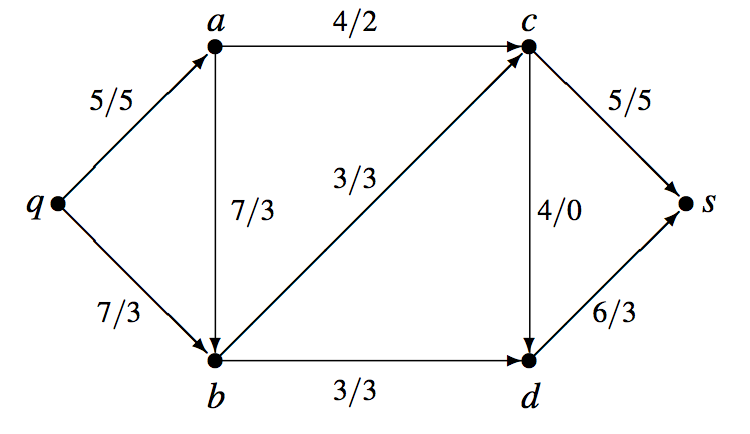
\includegraphics[width=4.5cm]{GraphZuResidual}
\item Bilde das Residualnetzwerk. ``Subtrahiere'' also die Kapazitäten die durch den ersten Fluss benutzt werden.
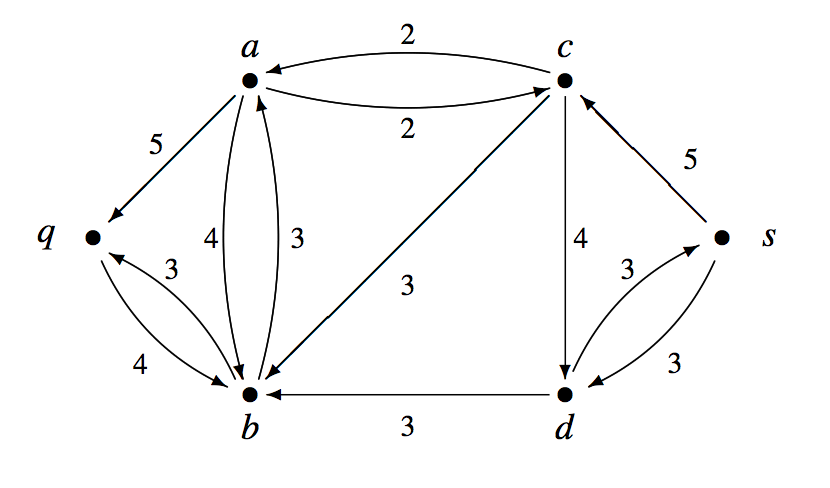
\includegraphics[width=5cm]{ResidualGraph}
\item Wähle einen Fluss im Residualnetzwerk, und wiederhole Schritte 2 und 3 bis kein weiterer Fluss existiert.
\end{enumerate}

\subsubsection{Edmonds und Karp}
Laufzeit: $\Oh(|V|*|E|^2)$
\subsubsection{Dinic}
Laufzeit: $\Oh(|V|^2*|E|)$

\subsection{Geometrische Algorithmen}
\subsubsection{Konvexe Hülle}
Die konvexe Hülle einer Menge von Punkten in der Ebene ist jenes Polynom, welches man erhält, wenn man eine Schnur straff um die Punkte spannt. D.h. wenn eine Gerade zwischen zwei Punkten alle anderen Punkte auf einer Seite hat, ist sie Teil der konvexen Hülle.

\paragraph{Jarvis' Marsch} ist die intuitive Technik, man startet an dem Punkt mit der kleinsten $x$-Koordinate, und `lässt die Schnur nach unten baumeln', und rotiert sie dann gegen den Uhrzeigersinn, bis man auf einen nächsten Punkt trifft. $\Oh(Nh)$, mit $h$ Anzahl Punkte auf der Hülle. Effizient, wenn die Hülle aus wenigen Punkten besteht, aber potentiell $\Oh(N^{2})$, z.B. bei einem Kreis.

\begin{center}
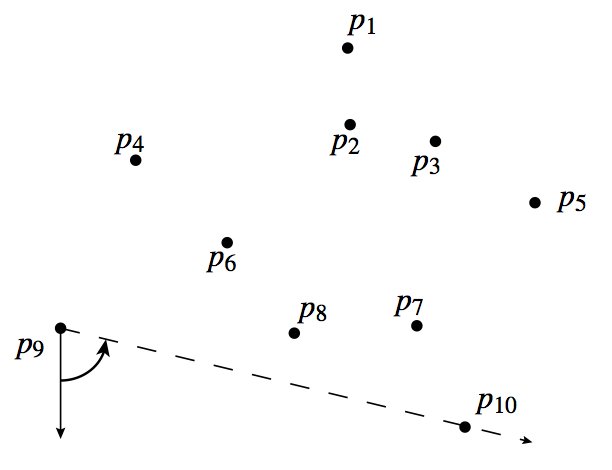
\includegraphics[width=6cm]{JarvisMarch}
\end{center}

\paragraph{Graham's Scan}
Wähle einen Punkt und errechne die $n-1$ Linien aus allen anderen Punkten. Sortiere zyklisch nach der Steigung (Winkel) und entferne schliesslich alle ``Links-Knicke''. Amortisierte Laufzeit $\Oh(n\log{n})$.
\begin{center}
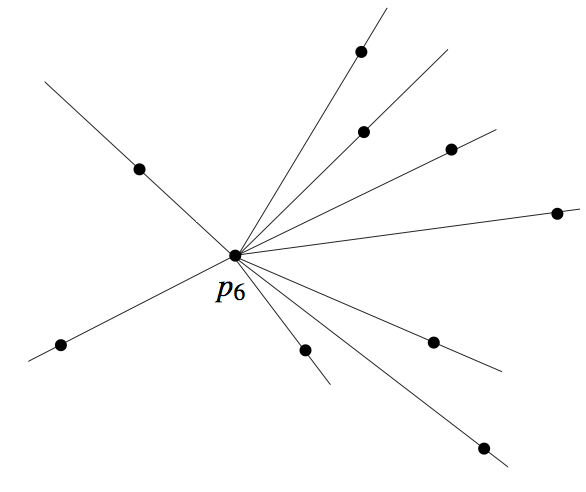
\includegraphics[width=2.8cm]{GrahamScan1}
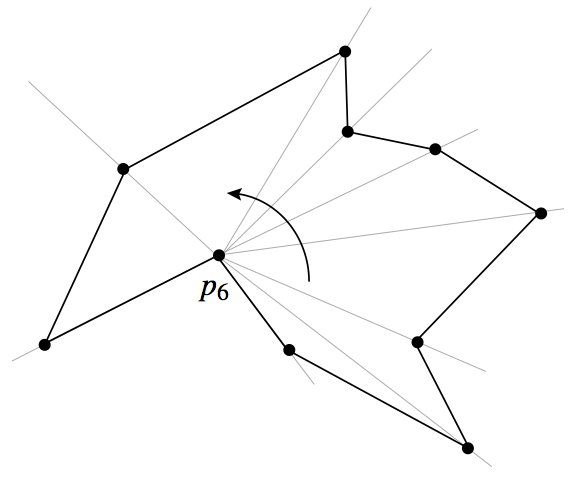
\includegraphics[width=2.8cm]{GrahamScan2}
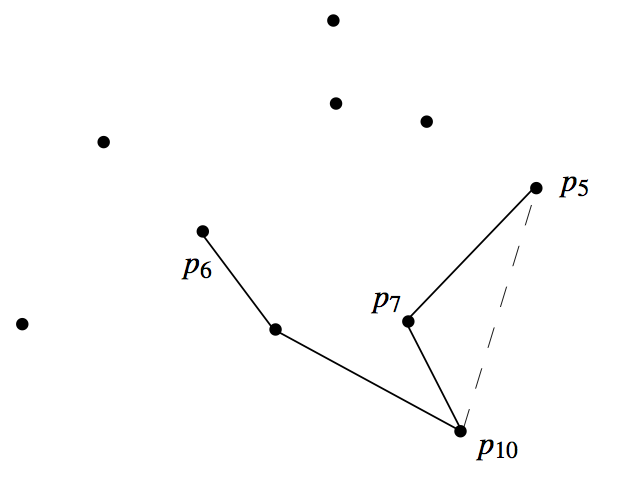
\includegraphics[width=2.8cm]{GrahamScan3}
\end{center}

\subsubsection{Scan-line-Prinzip}
Eine Beschreibung eines Scanline-Algorithmus muss immer folgende Punkte beinhalten:
\begin{enumerate}
\item \emph{Haltepunkte.} In welcher Richtung verläuft die Scanline? Was sind die Haltepunkte?
\item \emph{Scanline-Datenstruktur.} Welche Objekte muss die Datenstruktur verwalten? Welche Operationen müssen unterstützt werden? Was ist eine angemessene Datenstuktur?
\item \emph{Aktualisierung.} Was passiert, wenn die Scanline auf einen Haltepunkt trifft? 
\item \emph{Auslesen der Lösung.} Wie lässt sich die Lösung auslesen?
\end{enumerate}

\section{Datenstrukturen}
\subsection{Listen}

\subsubsection{Selbstanordnende Listen}
Sind nützlich bei grossen Unterschieden in der Zugriffshäufigkeit auf Elemente, dann lohnt es sich nämlich, die häufiger genutzten möglichst weit vorne zu platzieren.
\begin{description}
\item[Move-to-front] bedeutet, dass ein gebrauchtes Element an den Anfang verschoben wird. Die restliche Ordnung verändert sich nicht. Asymptotisch optimal.
\item[Transpose] heisst schlicht dass ein abgerufenes Element einen Platz nach vorne rutscht.
\end{description}

\paragraph{Frequency Count} ordnet jedem Element einen Zähler zu, und ordne nach jedem Zugriff die Liste nach dem Zähler.

\subsubsection{Skip-Listen}
\paragraph{Randomisierte Skip-Listen}
Eine randomisierte Datenstruktur, bestehend aus verschiedenen Ebenen. Die unterste Ebene ist eine normale verkettete Liste. Die höheren Ebenen kann man sich als Überholspur vorstellen. Ein Element wird in der untersten Ebene eingefügt, und dann mit gewissen Wahrscheinlichkeiten $p$ in die Ebenen darüber eingefügt.

\paragraph{Perfekte Skip-Liste}
Die perfekte Skip-Liste hat ebenfalls eine verkettete Liste als Niveau 0. Dazu kommt aber, dass jedes $2^{i}$-te Element eine Zeiger das Element $2^{i}$ Positionen weiter hat, für $i=0,\dots,\floor{\log{N}}$. Es hat also im Niveau 1 die Elemente $2,4,6,\dots$, im Niveau 2 die Elemente $4, 8, 12$ etc.


\subsection{Heaps - ``Halden'' :D}
\begin{description}
\item[Max-Heapbedingung] besagt $k_{i}\leq k_{\floor{\frac{i}{2}}}$ für $2 \leq i \leq N$.
\item[Min-Heapbedingung] besagt $k_{i}\geq k_{\floor{\frac{i}{2}}}$ für $2 \leq i \leq N$.
\end{description}
Jeder Schlüssel ist kleiner (grösser) als der Vaterschlüssel. \\
Bei einem Min-(Max-)Heap kann das Minimum (Maximum) in einem Schritt bestimmt werden.

\subsubsection{Binomial-Heap}
Der Binomial-Heap, eine Priority-Queue, besteht aus Listen von Binomial-Bäumen verschiedener Ordnung. 
\paragraph{Der Binomial-Baum} ist rekursiv definiert:
\begin{itemize}
\item Ein Binomial-Baum der Ordnung 0 besteht aus einem einzenen Knoten.
\item Ein Binomial-Baum der Ordnung k besitzt eine Wurzel mit Grad $k$ deren Kinder genau die Ordnung $k-1, k-2, \dots, 0$ besitzen.
\end{itemize}
\begin{center}
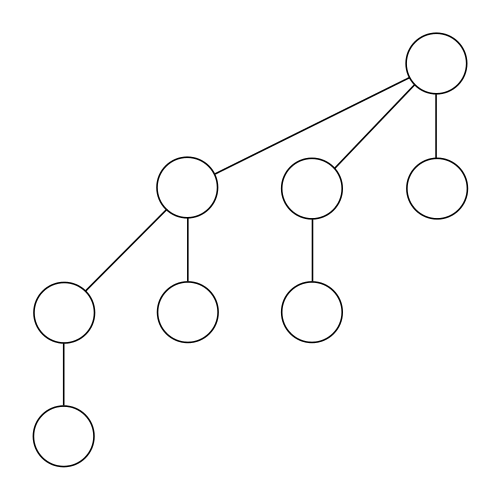
\includegraphics[width=6cm]{BinomialTree3}

Ein Binomial-Baum mit Ordnung 3
\end{center}

In einem Binomial-Heap gelten folgende Bedingungen. \begin{itemize}
\item Die Heap-Bedingung: Jeder Schlüssel ist kleiner als sein Vorgänger.
\item Für jede natürliche Zahl $k$ gibt es nur einen Binomial-Baum der Ordnung $k$
\end{itemize}
Ein Binomial-Heap unterstützt die folgenden Operationen.
\begin{description}
\item[insert] -- Einfügen
\item[remove] -- Löschen
\item[extractMin] -- Rückgabe und Entfernung vom Element mit dem minimalen Schlüssel, also der höchsten Priorität
\item[changeKey] -- zum Ändern des Schlüssels eines Elements.
\item[merge] -- Vereinigung von zwei Binomial Heaps. 
\end{description}
Alle diese Operationen können in einer \emph{Worst-Case-Zeit} von $\Oh(\log{n})$ implementiert werden. 

\subsubsection{Fibonacci-Heap} Der Fibonacci-Heap ist vom Binomial-Heap abgeleitet, also auch eine Priority-Queue. Ein F-Heap ist eine Kollektion heap-geordneter Bäume mit disjunkten Schlüsselmengen. Alle Operationen ausser $extractMin$ ($\Oh(\log{n})$) lassen sich in amortisiert $\Oh(1)$ implementieren. 

\begin{center}
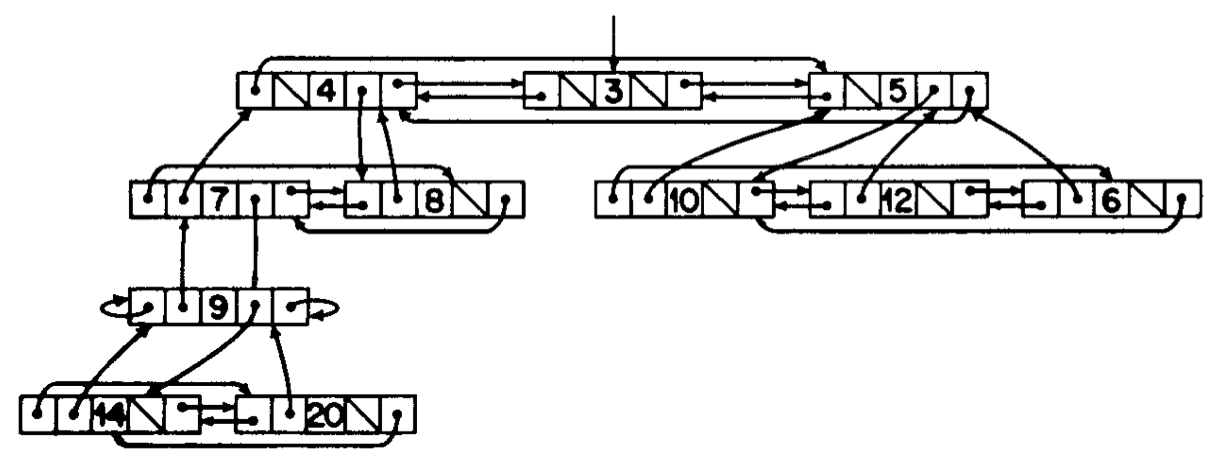
\includegraphics[width=\linewidth]{FibonacciHeap}

Ein Fibonacci Heap mit Pointern, aber ohne Markierung
\end{center}
Jeder Knoten hat einen Pointer auf sein linkes Geschwister, sein Elternteil, ein Kind und das rechte Geschwister. Das mittlere Feld ist der Schlüssel. Es ist ein Markierungsbit in jedem Knoten vorhanden. Die Kinder eines Knotens sind in einer verketteten zyklischen Liste gespeichert. Der Rang eines Knotens ist die Anzahl seiner Kinder.

\paragraph{Operationen auf dem Fibonacci Heap} 
\begin{description}
\item[makeHeap()] Gibt einen Pointer auf den Null-Knoten zurück.
\item[findMin($h$)] Es gibt einen Pointer auf das minimale Element von $h$, also ist $findMin$ trivial.
\item[extractMin($h$)] Die schwierigste Operation. Wir beginnen indem wir das minimale Element $x$ von $h$ entfernen, die Liste der Kinder von $x$ und die der Wurzeln ausser $x$ verketten und wiederholen dann den folgenden Schritt bis er nicht mehr anwendbar ist:
\begin{itemize}[leftmargin=*]
\item
\emph{Linking Step}. Finde zwei Bäume deren Wurzel denselben Rang hat, und verschmelze sie. (Der neue Baum hat jetzt einen höheren Rang als die Ränge der verschmolzenen).
\end{itemize}
Sobald keine Bäume mit dem selben Rang übrig sind bilden wir eine Liste aus den übrigen Wurzeln, wobei wir auch das neue Minimalelement finden.
\item[insert($i,h$)] Wir kreieren einen neuen Heap mit $i$ als einzigem Element und rufen $meld(h, h_{\text{neu}})$ auf.
\item[meld($h_{1}, h_{2}$)] Wir vereinigen die Wurzellisten von $h_{1}$ und $h_{2}$ und bestimmen das Minimum aus den beiden vorherigen Minimas.
\item[decreaseKey($\Delta,i,h$)] Wir subtrahieren $\Delta$ von $i$, finden den Knoten $x$ der $i$ enthält und entfernen die Kante zwischen $x$ und seinem Elternteil $p(x)$. Wir entfernen also den Parent-Pointer von $x$ auf $p(x)$ und löschen $x$ aus der Liste der Kinder von $p(x)$. Damit haben wir den Teilbaum mit $x$ als Wurzel zu einem neuen Baum in $h$ gemacht, und müssen noch überprüfen, ob $x$ das neue Minimalelement ist.
\item[delete($i,h$)] Finde den Knoten $x$ der $i$ enthält, entferne die Kante zu $p(x)$. Erstelle eine neue Wurzelliste durch verketten der Kinder von $x$ mit der alten Wurzelliste.
\end{description}
Ein wichtiges Detail ist noch zu beachten. Nachdem Knoten $x$ zum Kind eines anderen Knoten gemacht wurde, sobald $x$ zwei seiner Kinder verliert, entfernen wir die Kante zwischen $x$ und $p(x)$. Wir nennen diesen Schnitt \emph{Cascading Cut}, Kaskadierender Schnitt. Dies ist auch der Sinn der Markierungen. Wenn $x$ Kind eines anderen Knoten wird, unmarkieren wir $x$. Wenn wir eine Kante zwischen $x$ und $p(x)$ entfernen, und $p(x)$ keine Wurzel ist, markieren wir $p(x)$ falls er noch nicht markiert ist, und entfernen die Kante zu \emph{seinem} Elternteil.
Bleh.

\subsection{Bäume}
Bäume sind verallgemeinerte Listen, in denen jedes Element (Knoten) eine begrenzte Anzahl Söhne haben kann. Keine Duplikate! 

\subsubsection{Traversierung von Binärbäumen}
\begin{description}
\item[Preorder] Wurzel, Linker Teilbaum, Rechter Teilbaum
\item[Postorder] Linker Teilbaum, Rechter Teilbaum, Wurzel
\item[Inorder] Linker Teilbaum, Wurzel, Rechter Teilbaum
\end{description}

\subsubsection{Vanilla Binärsuchbaum} mit einer Wurzel, und grösseren rechten Nachfolgern, kleineren linken Nachfolgern.
\begin{description}
\item[Suchen] Rekursiv in Teilbäumen $T$. Abbruch wenn $T$ keine Wurzel ist. Wenn $x <$ Wurzel von $T$ suche in linkem Teilbaum, sonst im rechten.
\item[Einfügen] Suchen nach Knoten, einfügen als Blatt des Knoten in dem die Suche endete.
\item[Löschen] Wenn Blatt, löschen. Wenn einen Sohn, löschen und Sohn hochziehen. Wenn zwei Söhne, symmetrischer Nachfolger suchen und zu löschender Knoten ersetzen.
\end{description}

\subsubsection{AVL-Bäume} sind balancierte binäre Suchbäume. In jedem Knoten muss gelten: Der Höhenunterschied zwischen dem rechten Teilbaum und dem linken Teilbaum ist höchstens 1.
\begin{description}
\item[Suchen] Genau wie bei einem normalen binären Suchbaum.
\item[Einfügen] Wie bei einem normalen Binärsuchbaum, aber dann Balanceinformationen erneuern. Falls Höhenunterschied zu gross: Einfach- oder Doppelrotation bis wieder balanciert, dann weiter Balanceinformationen erneuern.
\item[Löschen] Wie beim BSB, aber danach wieder balancieren.
\end{description}
\paragraph{Rotationen}
\begin{enumerate}
\item Den unbalacierten Knoten rot färben.
\item Dessen schweres Kind grün färben.
\item Fallunterscheidung:
\begin{enumerate}
\item Die Kinder des grünen Knoten sind gleich schwer: \emph{Einfachrotation}
\item Sonst das schwere Kind des grünen Knoten blau färben:
\begin{itemize}
\item Falls rot $<$ grün $<$ blau oder rot $>$ grün $>$ blau: \emph{Einfachrotation}
\item Sonst: \emph{Doppelrotation}
\end{itemize}
\end{enumerate}
\end{enumerate}


%\paragraph{Huffman-Baum} wird erstellt durch die Huffman-Kodierung, ein Kompressionsverfahren. Die Mächtigkeit des Alphabets über dem kodiert wird heisst $m$. Man kreiert einen Wald, der aus den verwendeten Zeichen und ihren Häufigkeiten besteht. Dann nimmt man die geringsten $m$ Häufigkeiten und addiert sie, und verschmilzt sie zu einem Baum (der Ordnung $m$) mit der Summe als Wurzel. Dann nimmt man wieder die zwei kleinsten Häufigkeiten, was (beim Binäralphabet) die Summe und ein neues Element oder zwei neue Elemente sein kann.

\subsubsection{Optimale Suchbäume} versuchen die (erwarteten) Suchkosten zu minimieren.
\begin{description}
\item[Die Menge $S=k_{1}, \dots, k_{n}$] von $n$ verschiedenen Schlüssel,
\item[Die Häufigkeit $a_{i}$] mit der nach $k_{i}$ gesucht wird,
\item[Das offene Interval $(k_{0}, k_{n+1})$] von Schlüsseln, nach denen gesucht werden kann (Oft gilt $k_{0}=-\infty$ und $k_{n+1}=\infty$),
\item[Die Häufigkeit $b_{j}$] mit der nach einem Schlüssel $x\in (k_{j}, k_{j+1})$ gesucht wird.
\item[Das Gewicht $W$] des Suchbaums die summierte Häufigkeit seiner Knoten: $W=\sum_{i}{a_{i}}+\sum_{j}{b_j}$
\item[Die gewichtete Pfadlänge $P$] misst wie viele Schlüsslvergleiche total nötig sind: \[P= \sum^{n}_{i=1}{(\text{depth}[k_{i}]+1})*a_{i}+\sum^{n}_{j=0}{\text{depth}(\text{leaf}(k_{j}, k_{j+1}))*b_{j}}\]
\end{description} 
\begin{center}
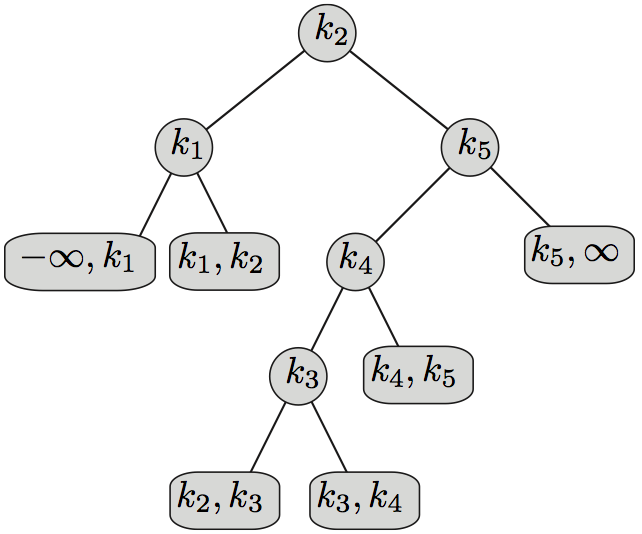
\includegraphics[width=6cm]{OptimalerSuchbaum}
\end{center}

Ein Suchbaum heisst optimal, wenn $P$ minimal ist. Es gilt, dass jeder Teilbaum eines optimalen Suchbaums auch ein optimaler Suchbaum ist. Somit eignet sich die dynamische Programmierung für einen Algorithmus.


\paragraph{Splay-Bäume}
Splay-Bäume sind reine binäre Suchbäume, die sich durch eine Variante der Move-To-Root Strategie selbst anordnen. Alle Standard-Operationen haben eine amortisierte Laufzeit von $\Oh(\log{n})$. Die \emph{splay}-Operation ist wiefolgt definiert:
\begin{itemize}
\item (zig) Wenn $p(x)$, der Vater von $x$, die Wurzel ist, rotiere die Kante welche $x$ mit $p(x)$ verbindet. (terminal case)
\item (zig-zig) Wenn $p(x)$ \emph{nicht} die Wurzel ist und $x$ und $p(x)$ beides rechte oder linke Kinder sind, rotiere die Kante welche $p(x)$ mit dem Grossvater $g(x)$ verbindet, und rotiere dann die Kante welche $x$ mit $p(x)$ verbindet. 
\item (zig-zag) Wenn $p(x)$ \emph{nicht} die Wurzel ist und $x$ ein linkes, $p(x)$ ein rechtes Kind sind, rotiere die Kante welche $x$ mit $p(x)$ verbindet, und dann die Kante, welche $x$ mit dem neuen $p(x)$ verbindet.
\end{itemize}


\subsubsection{B-Baum}
Nützlich, wenn nicht der ganze Baum im Hauptspeicher Platz hat. Ein B-Baum der Ordnung $m$ ist ein Baum mit den folgenden Eigenschaften:
\begin{enumerate}
\item Alle Blätter haben die gleiche Tiefe.
\item Jeder Knoten mit Ausnahme der Wurzel und der Blätter hat wenigstens $\ceil{\frac{m}{2}}$ Söhne
\item Die Wurzel hat wenigstens 2 Söhne.
\item Jeder Knoten hat höchstens $m$ Söhne.
\item Jeder Knoten mit $i$ Söhnen hat $i-1$ Schlüssel
\end{enumerate}

\begin{center}
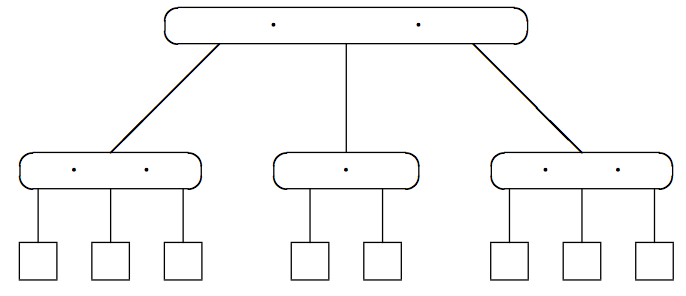
\includegraphics[width=5cm]{B-Baum}

Ein B-Baum der Ordnung 3
\end{center}

\subsection{Scanline Datenstrukturen}

Eine Überlappungsanfrage ist äquivalent zu einer Aufspiessanfrage und einer Bereichsanfrage. Um eine Überlappung mit $[a,b]$ zu prüfen, genügt es also
\begin{enumerate}
\item alle Intervalle $[a',b']$ zu finden, die der linke Randpunkt $a$ aufspiesst und
\item alle Intervalle $[a',b']$ zu finden, deren linker Randpunkt $a'$ im Bereich $[a,b]$ liegt.
\end{enumerate}

\subsubsection{Segment-Bäume}
Konstruiert von einem vollständigen Binärbaum, der alle elementaren Segmente als Blätter hat. See Pic :]

\begin{description}
\item[delete] braucht Wörterbuch mit den Intervallen. Dann $\Oh(\log{n})$.
\item[insert]ist in $\Oh(\log{n})$ Schritten ausführbar.
\item[Aufspiessanfragen]brauchen $\Oh(\log{n}+k)$ mit $k$ als Grösse der Antwort. Eine Aufspiessanfrage nach $x$ wird realisiert indem der Segment-Baum als Suchbaum für $x$ benutzt wird, d.h. wir suchen das Elementarsegment welches $x$ beinhaltet. Dann geben wir als Antwort alle Listen von Intervallen an, die wir in den Knoten auf dem Weg angetroffen haben.
\end{description}

\begin{center}
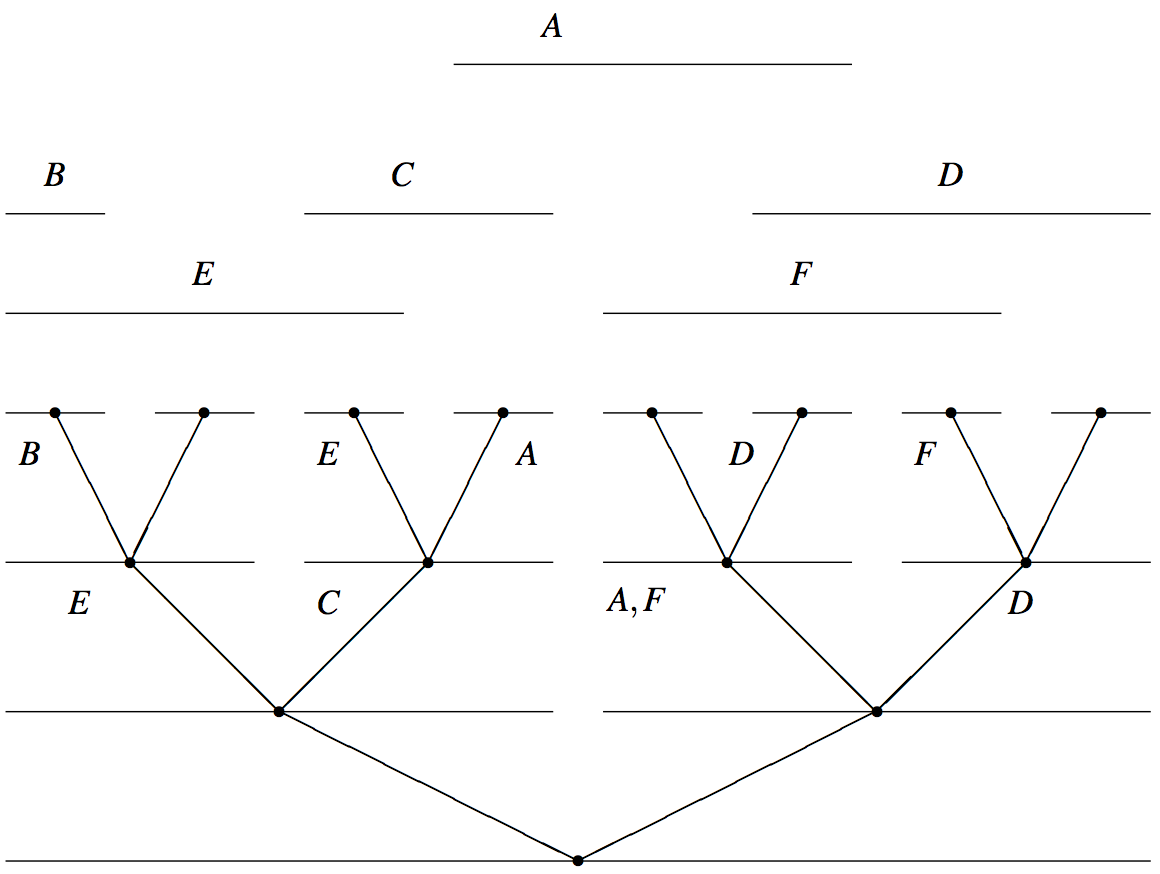
\includegraphics[width=6cm]{SegmentBaum}

Ein Segment Baum
\end{center}

\subsubsection{Intervall-Bäume}
In einem Intervall-Baum hat jeder Knoten zwei verkettete Listen von Intervallen, die $u$- und die $o$-Liste. Die $u$-Liste ist eine nach aufsteigenden unteren Endpunkten sortiert, die $o$-Liste nach absteigenden oberen Endpunkten. Ein Intervall $[l, r]$ kommt in beiden Listen  desjenigen Knotens im Skelett des Intervall-Baumes mit minimaler Tiefe vor, dessen Schlüssel im Intervall $[l,r]$ liegt. \\
Für die Menge der Intervalle $\{[1,2],[1,5],[3,4],[5,7],[6,7],[1,7]\}$ haben wir demnach den folgenden Intervall-Baum:

\begin{center}
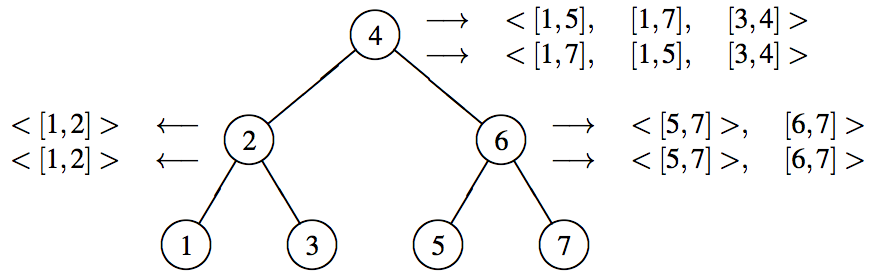
\includegraphics[width=7cm]{IntervallBaum}
\end{center}

\begin{description}
\item[delete] ist in $\Oh(\log{n})$ Schritten ausführbar.
\item[insert] ist in $\Oh(\log{n})$ Schritten ausführbar.
\item[Aufspiessanfragen] brauchen $\Oh(\log{n}+k)$ mit $k$ als Grösse der Antwort.	
\end{description}

\subsubsection{Prioritäts-Suchbäume}
sind 1.5-dimensional, und speichern 2-dimensionale Daten. Jeder Punkt $(x,y)$ (also jedes Intervall $[x,y]$) wird auf einem Suchpfad von der Wurzel zum Blatt $x$ an einem inneren Knoten entsprechend seinem $y$-Wert abgelegt. Wir haben also gleichzeitig einen Min-Heap über $y$ und einen BSB über $x$. Mit $A,B,C,D$ wie angegeben:

\begin{center}
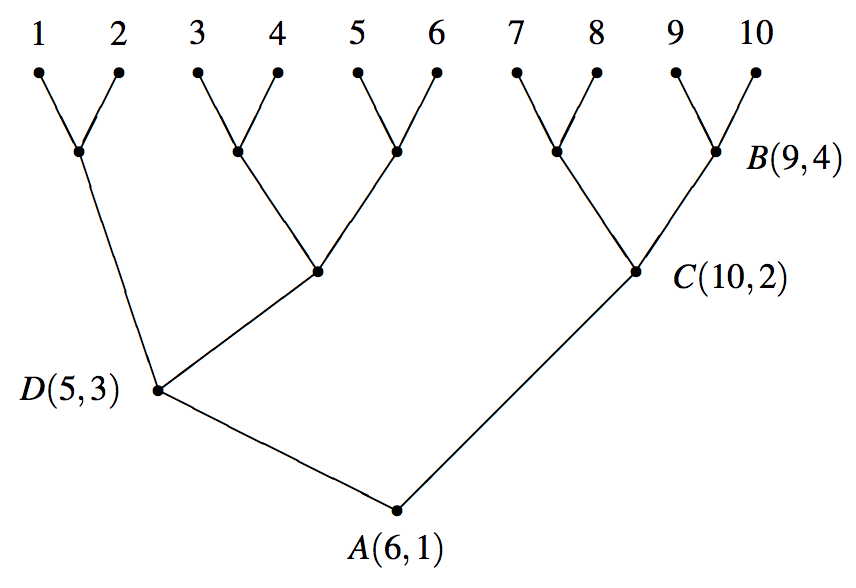
\includegraphics[width=7cm]{PrioritaetsSuchBaum}
\end{center}

\begin{description}
\item[insert] wird am Anfang immer in die Wurzel gehen, dann dem Suchbaum folgen.
\item[delete] sucht zuerst nach dem zu löschenden Punkt, und dann der Sohn mit dem kleineren $y$-Wert hochgezogen (um die Heap-Bedingung nicht zu verletzen).
\item[Bereichsanfrage] in $\Oh(\log{n}+k)$ Schritten.
\end{description}

Es gibt auch eine Möglichkeit, den Prioritäts-Suchbaum voll dynamisch zu realisieren, siehe S.524 in Widmayer.

\subsection{Union-Find-Struktur}
Der einfachste Weg das Union-Find-Problem zu lösen, ist jede Kollektion $K$ als ein unsortierter Baum beliebiger Ordnung darzustellen. Dabei ist die Wurzel des Baumes das kanonische Element. Union-Find-Strukturen unterstützen die folgenden drei Operationen:
\begin{description}
\item[Make-set($e,i$)] kreiert aus dem einzigen Element $e$ eine Menge $i$. Es wird vorausgesetzt, dass $e$ in keiner anderen Menge vorkommt. $\Oh(1)$
\item[Find($x$)] findet den Namen $i$ der Menge, die $x$ enthält.
\item[Union($i,j,k$)]  vereinigt die Mengen $i, j$ zu $k$. $i$ und $j$ werden aus der Kollektion der Mengen entfernt, $k$ hinzugefügt. $\Oh(1)$
\end{description}

\paragraph{Vereinigung nach Höhe} nennt sich das Verfahren, den weniger hohen Baum an den höheren Baum zu hängen.

\section{Graphen}
Ein Graph besteht aus einer Knotenmenge $V$ (vertices) und einer Menge $E \subseteq {V \choose 2}$ von geordneten (gerichtet) oder ungeordneten (ungerichtet) Paaren von \emph{Knoten} aus $V$, genannt \emph{Kanten}.
\begin{description}
\item[DAGs] sind directed acyclic graphs, also gerichtete zyklische Graphen. Sie treten oft in Schedulingproblemen auf. (Siehe Dynamisches Programmieren)
\item[Topologische Sortierungen] sind Ordnungen über DAGs, die, wenn z.B. eine Kante von $x$ nach $y$ heisst, dass $x$ vor $y$ eintreten muss, einem zeitlich sinnvollen Ablauf entspricht. Damit eine topologische Sortierung existieren kann, ist $\frac{n(n-1)}{2}$ die maximale Anzahl Kanten.
\item[Matching] ist eine Menge von Kanten ohne gleiche Knoten. Ein maximales Matching ist ein Matching, welches mit der Hinzunahme irgendeiner Kante nicht mehr ein Matching ist.
\end{description}

\subsection{Repräsentationen eines Graphen}
\begin{description}
\item[Adjazenzlisten] sind Listen für jeden Knoten, in dem die Nachbarn gespeichert werden. Für viele Fälle die bessere Wahl, abgesehen vom Löschen ($\Oh(d)$) und Testen ob eine Kante im Graph ist (auch $\Oh(d)$), wobei $d=$ Anzahl Nachbarn.
\item[Adjazenzmatrizen] sind $|V|\times|V|$ Matrizen, welche im Eintrag $(i,j)$ eine Eins speichern, falls es eine Kante von Knoten $i$ zu Knoten $j$ gibt. 
\end{description}

Algorthmen über Graphen: Kapitel \ref{graphalgos}, S. \pageref{graphalgos}

\subsection{Flüsse}
Im folgenden ist $G=(V,E)$ ein gerichteter Graph mit Kapazitätsfunktion $c: E\to\R$ und zwei ausgezeichneten Knoten, einer \emph{Quelle q} und einer \emph{Senke s}. Ein Fluss ist als eine Funktion $f: E\to\R^{+}_{0}$ definiert, wobei zwei Einschränkungen gelten:
\begin{description}
\item[Kapazitätsbeschränkung]
Für alle $e\in E$ ist $f(e)\leq c(e)$
\item[Flusserhaltung]
Für alle $v\in V - \{q,s\}$ gilt \[ \sum_{v',v\in E}{f((v',v))}-\sum_{v,v''\in E}{f((v,v''))} = 0\]
\end{description}

\begin{center}
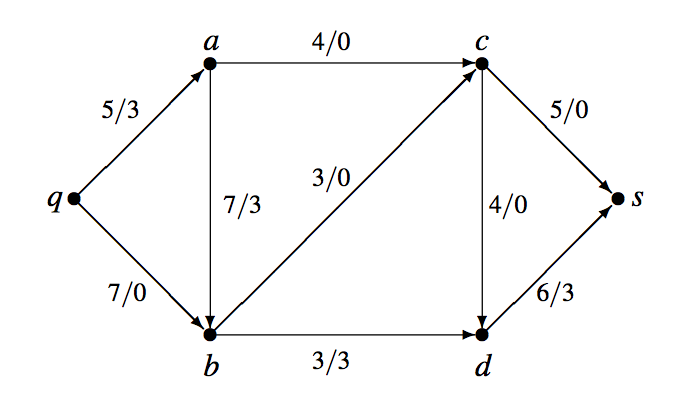
\includegraphics[width=6cm]{FlowExample}

Kapazität/Fluss
\end{center}

In diesem Beispiel fliesst ein Fluss von $q$ über $a,b,d$ zu $s$. Der \emph{Wert} $w(f)$ eines Flusses $f$ ist die Summe der Flusswerte aller $q$ verlassender Pfeile: $w(f) = \sum_{(q,v)\in E}{f((q,v))}-\sum_{(v',q)\in E}{f((v',q))}$. Oben also 3. Ein \emph{maximaler Fluss} in $G$ ist ein Fluss $f$ in $G$ mit maximalem Wert $f(f)$ unter allen Flüssen in $G$.
\subsubsection{Schnitte}
Ein \emph{Schnitt} ist eine Zerlegung von $V$ in zwei Teilmengen $Q,S$, so dass $q$ zu $Q$ und $s$ zu $S$ gehört. (Der Schnitt muss also $q$ und $s$ trennen). Die \emph{Kapazität} eines Schnittes ist die Summe der \emph{Kapazitäten} (egal wie viel fliesst) der Pfeile, welche von $Q$ nach $S$ führen (die Kapazitäten in die andere Richtung werden ignoniert.). Der Schnitt mit der kleinsten Kapazität heisst \emph{minimaler Schnitt}. Im Beispiel oben ist $Q = \{q,b\},\, S = \{a,c,d,s\}$ ein Schnitt mit Kapazität $11$. Es gilt: \emph{Min Cut = Max Flow}
Algorithmen über Flüsse: Kapitel \ref{flowalgos}, S. \pageref{flowalgos}

\section{Verschiedenes}

\subsection{Vollständige Induktion}
Kann für ein Prädikat $P(n)$ bewiesen werden, dass $P(n_0)$ und $\forall n\in\N: n > n_0 \wedge P(n) \to P(n+1)$ gilt,
dann folgt daraus $\forall n\in\N: n \geq n_0 \rightarrow P(n)$.

\paragraph{Induktionsannahme (IA)} bezeichnet das Prädikat $P(n)$.

\paragraph{Induktionsverankerung (IV)} ist der Beweis von $P(n_0)$.

\paragraph{Induktionsschritt (IS)} ist der Beweis von $P(n) \rightarrow P(n+1)$.

\subsection{Bitonische Läufe}\label{bitonische_laufe}
Bitonische Läufe, sind Folgen, die zuerst monoton steigen, dann monoton fallen (darum ``bi-tonisch'').
 \[ a_i \leq a_{i+1} \leq \dots \leq a_{i+m} \geq a_{i+m+1} \geq \dots \geq a_{j+k} \]

\subsection{Rekursionsgleichungen}
Ein paar mal in sich selbst einfügen, Pattern erkennen und auflösen. Sehr oft sind Terme wie $\displaystyle c*\sum^{\log_b{(n)}-1}_{i=0}{x^i}$ die sich dann zu $\displaystyle\frac{x^{\log_b{n}}-1}{x-1}$ vereinfachen. 


\end{document}
